\chapter*{Wstęp}
Częstym zadaniem tworzonego oprogramowania jest prezentacja pewnych danych. Nawet najlepszy program wykonujący skomplikowane obliczenia jest niewiele wart dla klienta, jeśli nie potrafi w~przystępny sposób zaprezentować efektów swoich działań.
 
Jedną z~podstawowych form prezentacji danych w~informatyce i~nie tylko jest tabela, która umożliwia wyświetlanie danych z~dużą precyzją. Qt posiada już architekturę służącą tworzeniu takich systemów -- Model-Widok. Jest to bardzo popularna platforma umożliwiająca tworzenie skomplikowanych interaktywnych tabelek prezentujących dane z~różnych źródeł, m.in. z~bazy danych.

Inną formą prezentacji danych są wykresy, których popularność jest porównywalna do tabel. Jest to forma dużo bardziej przystępna dla ludzkiej percepcji. Ułatwiają szybkie porównywanie wielu rekordów oraz wyznaczanie tendencji. Ponadto ich obrazkowa natura oraz możliwe animacje sprawiają, że jest to forma bardzo atrakcyjna dla końcowego użytkownika oprogramowania.
Qt posiada już kilka bibliotek służących tworzeniu wykresów, jednak nadal istnieje zapotrzebowanie na wartościowe rozwiązanie open-source, co wykażę w~rozdziale \textit{Przegląd dziedziny}.

W~rozdziale 2 omawiam dostępne biblioteki do tworzenia wykresów w~Qt. Następnie przedstawiam opis i~analizę wymagań stawianych mojej bibliotece. Kolejny rozdział to inżynierski projekt architektury całej biblioteki. Następne dwa rozdziały są poświęcone implementacji oraz testom biblioteki. Ostatni  zawiera wnioski dotyczące stworzonej biblioteki oraz możliwości jej dalszego rozwoju. 

\chapter{Wprowadzenie}
W~tym rozdziale przedstawiam podstawy Qt oraz Qt~Quick, dzięki którym dowolny czytelnik powinien zrozumieć zawartość mojej pracy.

\section{Qt}
Qt jest zbiorem bibliotek języka C++, które są dostępne na licencjach LGPL, GPL oraz komercyjnej. Lista bibliotek jest dość okazała, a~znaleźć na niej można narzędzia do tworzenia interfejsów użytkownika, parsowania plików XML czy dostępu do baz danych. Naczelną zasadą Qt jest: \textit{pisz raz, kompiluj wielokrotnie}~\footnote{\url{http://qt-project.org/wiki/QtWhitepaper}} -- dzięki takiemu podejściu programy napisane w~Qt są przenośne pomiędzy najpopularniejszymi platformami na poziomie kodu źródłowego.  


\subsection{Narzędzia}
Najważniejszymi narzędziami, które umożliwiają tudzież ułatwiają pracę z~Qt są:
\begin{itemize}
\item moc (Meta Object Compiler) -- specjalny program, który można porównać do preprocesora. Na podstawie naszego kodu generuje on dodatkowe pliki źródłowe potrzebne Qt, niewidoczne dla programisty.
\item uic (User Interface Compiler) -- kompilator plików *.ui, które zawierają informację o~układzie interfejsu użytkownika.
\item qmake -- program ułatwiający zarządzanie procesem budowania projektu.
\item Qt Creator -- zintergrowane środowisko programistyczne, przeznaczone głównie dla języków C++, QML i~JavaScript.
\item Qt Designer -- program umożliwiający łatwe tworzenie interfejsów użytkownika. Generuje on wspomniane juz pliki *.ui.
\end{itemize}


\subsection{QObject}
C++ nie wymusza dziedziczenia po określonej klasie, jak ma to miejsce chociażby w~Javie, gdzie zawsze na szczycie drzewa dziedziczenia znajduje się klasa \textit{Object}. Qt wprowadza swoją klasę -- \textit{QObject}. Dzięki wielodziedziczeniu, nie musimy rezygnować z dotychczasowej hierarchii dziedziczenia, aby otrzymać wiele ciekawych możliwości płynących z~wykorzystania \textit{QObject}.
Niektóre z~nich to:
\begin{itemize}
\item Relacja rodzic--dziecko, która jest nawiązywana w chwili tworzenia obiektów. Umożliwia ona wyszukiwanie dzieci danego obiektu po ich klasie, bądź nazwie. Ponadto ułatwia zarządzanie pamięcią, poprzez automatyczne usuwanie obiektów -- dzieci w chwili usunięcia rodzica. Przykład: usunięcie okna zawierającego wiele elementów spowoduje posprzątanie ze sterty wszystkich przycisków, etykiet czy obrazków.
\item \textit{qobject\_cast} -- dynamiczne rzutowanie, stosowane do rzutowania w dół hierarchii dziedziczenia. Jest ono znacznie szybsze od \textit{dynamic\_cast}, gdyż nie korzysta z mechanizmu RTTI (Run Time Type Information). Jedynym oczywistym mankamentem jest fakt, że rzutowanie to działa jedynie dla klas dziedziczących po \textit{QObject}.
\item Zdarzenia -- niskopoziomowy mechanizm komunikacji. Qt opakowuje standardowe zdarzenia w obiekty swoich klas i~dostarcza je do odpowiednich obiektów. Przed dostarczeniem zdarzenia do adresata można je przefiltrować, podejrzeć lub wręcz zmienić.
\item Sygnały i~sloty -- wysokopoziomowy mechanizm komunikacji będący implementacją wzorca \textit{Obserwator}~\cite{Patterns}.
Jest to bardzo wygodny sposób na luźne wiązanie obiektów, które mogą ze sobą współpracować, nie wiedząc nawzajem o swoim istnieniu.
\item Właściwości -- sposób na parametryzowanie obiektów. Istnieją zarówno właściwości statyczne, dodawane w czasie kompilacji, wspólne dla wszystkich obiektów danej klasy, np. wysokośc czy kolor, jak i~dynamiczne, przypisywane pojedynczym obiektom już w czasie wykonania programu.
\end{itemize}

\section{Qt Quick}
Qt~Quick jest nową technologią tworzenia GUI. Jej przeznaczeniem jest tworzenie lekkich, intuicyjnych oraz płynnie działających interfejsów, głównie na platformach mobilnych. W przeciwieństwie do tradycyjnego Qt, Qt~Quick nie wymaga znajomości C++, co ma dopuścić do pracy nad GUI nie tylko programistów, ale również projektantów -- grafików.
Na Qt~Quick składają się:
\begin{itemize}
\item QML -- deklaratywny język,
\item JavaScript -- imperatywny język,
\item Środowisko uruchomieniowe zintegrowane z Qt,
\item Designer,
\item API C++ umożliwiające integrację z aplikacjami Qt.
\end{itemize}

W Qt4, Qt~Quick był oparty na architekturze \textit{Graphics View}~\footnote{Framework Graphics View  \url{http://qt-project.org/doc/qt-5.0/qtwidgets/graphicsview.html}}, jednak problemy wydajnościowe zmusiły projektantów do sięgnięcia po bardziej zaawansowane narzędzia. W Qt5 wykorzystano bezpośrednio \textit{OpenGL} oraz \textit{SceneGraph}~\footnote{Scene Graph\url{http://en.wikipedia.org/wiki/Scene\_graph}}.

\subsection{QML}
QML (Qt Modeling Language) jest deklaratywnym językiem służącym głównie do opisu wyglądu i~zachowania GUI. QML może jednak służyć do zupełnie innych zastosowań. W~nowym systemie zarządzania procesem budowania projektów napisanych w~Qt -- QBS~\footnote{Qt Build Suit \url{http://qt-project.org/wiki/qbs}} językiem opisu projektu jest właśnie QML.

Relacja rodzic-dziecko elementów QML została zorganizowana w~drzewiastą strukturę, ułatwiającą zarządzanie elementami. Podobnie jak obiekty w~klasycznym Qt, elementy są parametryzowane poprzez  właściwości, np. id lub szerokość. 

Ciekawą cechą QML jest system wiązania wartości ze zmienną, który umożliwia uzależnienie zmiennej A~od zmiennej~B. Zmiana wartości zmiennej B~w~czasie wykonywania programu spowoduje automatyczne przeliczenie wartości zmiennej~A.

Elementy QML mogą być rozszerzane przez kod napisany w~JavaScript lub poprzez integrację z modułami napisanymi w~C++.

\subsection{Przykładowy kod QML}

\begin{lstlisting}[caption=Przykład QML, label=code:qml]
Item {
	width: 400
	height: 200

	Rectangle {
		id: rect
		x: 100; y: 50;
		width: height / 2; height: parent.height
		anchors.centerIn: parent
		color: "lightblue"
	}
}
\end{lstlisting}

Wykonanie powyższego kodu spowoduje wyświetlenie okienka z~rysunku~\ref{rys:qml}. Główny element posiada dziecko będące prostokątem o~takiej samej wysokości i~szerokości równej połowie jego wysokości. Ponadto prostokąt ten jest wyśrodkowany w~swoim rodzicu oraz ma jasnoniebieski kolor.

Jak widać dziecko może odwoływać się do swego rodzica za pomocą słowa \textit{parent}. Z~kolei inne elementy mogą się odwoływać do danego elementu za pomocą jego właściwości -- id.

\begin{figure}[H]
\centering
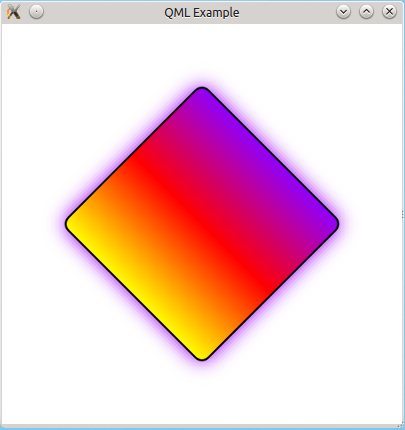
\includegraphics{img/qml.png}
\caption{Przykład wykorzystania QML}\label{rys:qml}
\end{figure}

\subsection{Własne elementy}
Istnieje możliwość tworzenia własnych elementów składających się z~elementów już dostępnych w~QML. Jednak bardzo złożone elementy, np. wykresy, łatwiej jest stworzyć w~C++, a następnie wyeksponować w~QML. Możliwe jest eksponowanie pojedynczych obiektów, jak i~eksportowanie całych klas. Aby klasa była zdatna do wykorzystania w~QML musi dziedziczyć po \textit{QObject}. Wyeksportowanie klasy odbywa się poprzez wywołanie jednej globalnej funkcji dostarczanej przez Qt. W~ten sposób zintegrowano z~QML chociażby bibliotekę Box2D.

